\documentclass[{../../master}]{subfiles}
\graphicspath{{../..}}  % 個別コンパイル時の画像パスを解決する

\begin{document}

本章では,ROSにおいてロボットの構造をモデリングするためのフォーマットであるURDF(Unified Robot Description Format)と,
URDFをプログラマブルに記述することのできるマクロパッケージである\textsf{xacro}\footnote{\url{http://wiki.ros.org/xacro}}について解説します.

\section{URDFとは?}

URDFについての説明をMathWorksのWebサイトから引用します.\cite{what_is_urdf}

\begin{quote}
  URDF (Unified Robotics Description Format) は、製造業の組み立てライン用ロボット マニピュレーター アームや遊園地用のアニマトロニクス ロボットなどのマルチボディ システムをモデル化するために、学術界や産業界で使用される XML 仕様です。
\end{quote}

URDFでは,ロボットのモデルをリンク(Link)とジョイント(Joint)からなるツリー構造で表現します.
ボディやホイール,センサ等,駆動しないブロックをリンクとして扱い,リンクとリンクとの接続(固定,回転,直動,etc)をジョイントとして扱います.
URDFによってモデリングされたロボットは,最終的に図\ref{fig:urdf_tree}\cite{urdf_xml_model}のような構造になります.

\begin{figure}[ht]
  \centering
  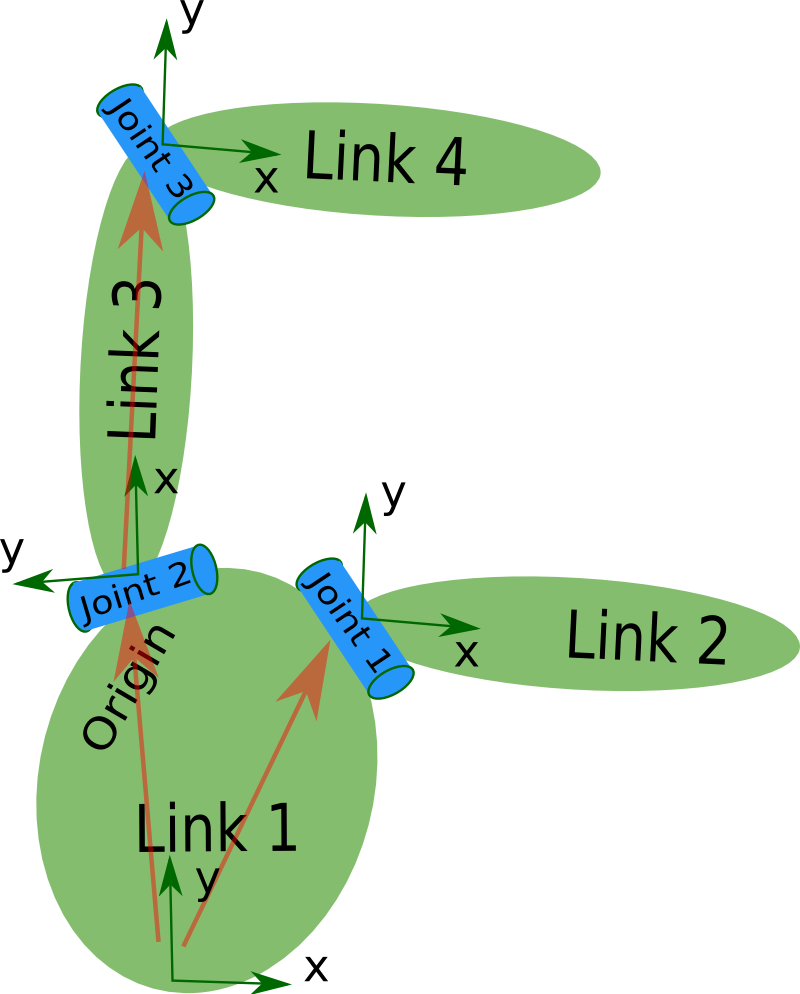
\includegraphics[width=70truemm, clip]{images/urdf_tree.png}
  \label{fig:urdf_tree}
  \caption{Tree Structure of URDF}
\end{figure}

URDFを記述することで,ロボットを構成する各リンクの位置関係やジョイントの属性を表すことができます.
また,URDFの各リンク/ジョイントに詳細なオプションを追加することで,シミュレーション用モデルを作成することもできます.

\end{document}